\documentclass[t,xcolor={svgnames,table}]{beamer}

\mode<presentation>
\usetheme{Warsaw}
\useoutertheme{infolines} 
\usepackage{natbib}
\usepackage{fontspec}
\usepackage{lmodern}
\usepackage{amsmath}
\usepackage{amsfonts}
\usepackage{bbm}
\usepackage{bm}
\usepackage[font=small,labelfont=bf]{caption} % Required for specifying captions to tables and figures
\usepackage{nicefrac}
\usepackage{color}
\usepackage{perpage}
\usepackage{multirow}
\usepackage{multicol}
\usepackage{adjustbox}
\usepackage{tikz}
\usepackage{tikz-dependency}
\usepackage{tikz-qtree}
\usepackage{tikz,pgfplots,pgfplotstable}
\usepackage{pgf}
\usepackage{collcell}
\usepackage{booktabs}
\usepackage{color,soul}

\usetikzlibrary{arrows.meta,graphs,graphs.standard,graphdrawing,quotes,shapes}
\usegdlibrary{layered,trees}

\tikzset{
  invisible/.style={opacity=0},
  visible on/.style={alt={#1{}{invisible}}},
  alt/.code args={<#1>#2#3}{%
    \alt<#1>{\pgfkeysalso{#2}}{\pgfkeysalso{#3}} % \pgfkeysalso doesn't change the path
  },
}

\captionsetup{labelformat=empty}

\newfontfamily\hebfont[Script=Hebrew, Scale=MatchUppercase]{FreeSans}
\newcommand{\heb}[1]{\bgroup\textdir TRT\hebfont #1\egroup}

\newcommand{\ucca}[1]{\textcolor{gray}{\textbf{\textsf{#1}}}}
\newcommand{\sst}[1]{\textsc{#1}}
\newcommand{\lexcat}[1]{\textsl{#1}}

\definecolor{orange}{rgb}{1,0.5,0}
\definecolor{mdgreen}{rgb}{0.05,0.6,0.05}
\definecolor{Acolor}{HTML}{EC5D57} % poppy red
\definecolor{Pcolor}{HTML}{70BF41} % grass green
\definecolor{Scolor}{HTML}{51A7F9} % sky blue
\definecolor{Lcolor}{HTML}{B36AE2} % friendly purple
\definecolor{mdblue}{rgb}{0,0,0.7}
\definecolor{dkblue}{rgb}{0,0,0.5}
\definecolor{dkgray}{rgb}{0.3,0.3,0.3}
\definecolor{slate}{rgb}{0.25,0.25,0.4}
\definecolor{gray}{rgb}{0.5,0.5,0.5}
\definecolor{ltgray}{rgb}{0.7,0.7,0.7}
\definecolor{purple}{rgb}{0.7,0,1.0}
\definecolor{lavender}{rgb}{0.65,0.55,1.0}


\makeatletter
\pgfdeclareshape{vector}{
      \inheritsavedanchors[from={rectangle}]
      \inheritbackgroundpath[from={rectangle}]
      \inheritanchorborder[from={rectangle}]
      \foreach \x in {center,north east,north west,north,south,south east,south west,east,west}{
        \inheritanchor[from={rectangle}]{\x}
      }

    \backgroundpath{
      \pgftransformshift{\pgfpoint{-16pt}{-4pt}}
          \draw[rounded corners=2pt] (0,0) rectangle (32pt,8pt);
    }

    \beforebackgroundpath{
      \draw[step=8pt,help lines,-] (8pt,.1pt) grid (24pt,7.9pt);
    }
}
\pgfdeclareshape{vector}{
      \inheritsavedanchors[from={rectangle}]
      \inheritbackgroundpath[from={rectangle}]
      \inheritanchorborder[from={rectangle}]
      \foreach \x in {center,north east,north west,north,south,south east,south west,east,west}{
        \inheritanchor[from={rectangle}]{\x}
      }

    \backgroundpath{
      \pgftransformshift{\pgfpoint{-16pt}{-4pt}}
          \draw[rounded corners=2pt] (0,0) rectangle (32pt,8pt);
    }

    \beforebackgroundpath{
      \draw[step=8pt,help lines,-] (8pt,.1pt) grid (24pt,7.9pt);
    }
}
\makeatother


% for confusion matrix
\newcommand{\ApplyGradient}[1]{%
  \pgfmathsetmacro{\PercentColor}{(#1-0)/63.88}%
  \pgfmathsetmacro{\PercentInverse}{ifthenelse(\PercentColor > 70, 0, 100)}%
  %\textcolor{black!\PercentColor}{#1}
  \edef\x{\noexpand\cellcolor{red!\PercentColor}}\x\textcolor{black!\PercentInverse}{#1}%
}
\newcolumntype{R}{>{\collectcell\ApplyGradient}{c}<{\endcollectcell}}


\MakePerPage{footnote}


\begin{document}


\title[]{Universal Meaning Representation and Parsing}
\author{Daniel Hershcovich}
\date{University of Copenhagen \\ Faculty of Science \\ December 19, 2019}

\begin{frame}
\titlepage
\end{frame}

\begin{frame}
\frametitle{What can we teach computers to do with language?}
\only<1>{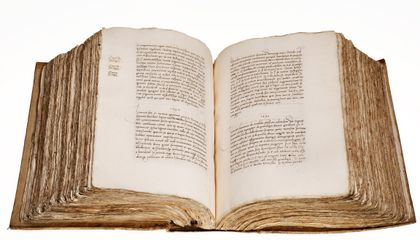
\includegraphics[width=\textwidth]{lostbook.jpg}}
\only<2>{Translate:}
\begin{center}
\onslide<2,6->{
  \fbox{\heb{דניאל עבר לקופנהגן אחרי שסיים את הלימודים}}
}

\only<2,4,5>{
  \fbox{After graduation, Daniel moved to Copenhagen}
}
\only<3,6->{
  \fbox{After graduation, \underline{Daniel} moved to \underline{Copenhagen}}
}
\end{center}

\vspace{-12mm}
  
\only<3>{
  Recognize \\ entities:

  \hspace{54mm} $\downarrow$ \hspace{27mm} $\downarrow$

  \hspace{49mm} Person \hspace{17mm} Location
}

\only<4>{
  \vspace{5mm}
  
  Infer:
}
  
\only<4>{
  \begin{center}
  $\downarrow$
  
  \fbox{Daniel graduated.}
  \end{center}
}

\only<5>{
  Simplify:
}
  
\only<5->{
  \vspace{6mm}
  
  \begin{center}  
  \fbox{Daniel graduated. Then Daniel moved to Copenhagen.}
  \end{center}
}

\only<2-5>{\vfill
\begin{center}

\includegraphics[width=.2\textwidth]{graduation.png}
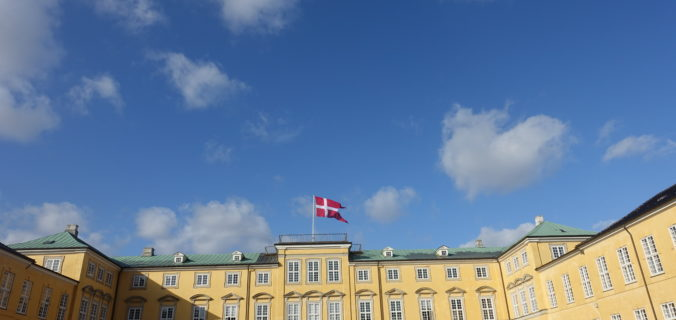
\includegraphics[width=.7\textwidth]{FRB-slot-676x320}
\end{center}}

\only<6->{
Identify relations between concepts (\textbf{parsing}, various frameworks):

    \begin{adjustbox}{center}
    \begin{dependency}[line width=2pt,label style={line width=.5pt,draw=black},opacity=.16]
        \begin{deptext}[column sep=1.5em,opacity=1]
          After \& graduation \& , \& Daniel \& moved \& to \& Copenhagen \\
        \end{deptext}
        \depedge[edge below,draw=DarkRed,edge unit distance=3ex]{1}{2}{ARG2}
        \depedge[edge below,draw=DarkRed,edge unit distance=3ex,opacity=1]{5}{4}{ARG1}
        \depedge[edge below,draw=DarkRed,edge unit distance=2ex, edge end x offset=-2pt]{1}{5}{ARG1}
        \deproot[edge below,draw=DarkRed,edge unit distance=3ex]{5}{top}
        \depedge[edge below,draw=DarkRed,edge unit distance=4ex, edge start x offset=-1pt, edge end x offset=3pt,opacity=1]{5}{7}{ARG2}
        \depedge[edge below,draw=DarkRed,edge unit distance=3ex, edge end x offset=5pt]{6}{5}{ARG1}
        \depedge[edge below,draw=DarkRed,edge unit distance=3ex]{6}{7}{ARG2}
        \depedge[draw=DarkBlue,edge unit distance=3ex]{2}{1}{case}
        \depedge[draw=DarkBlue,edge unit distance=3ex]{2}{3}{punct}
        \depedge[draw=DarkBlue,edge unit distance=3ex,opacity=1]{5}{4}{nsubj}
        \depedge[draw=DarkBlue,edge unit distance=3ex, edge end x offset=-2pt]{5}{2}{obl}
        \depedge[draw=DarkBlue,edge unit distance=3ex]{7}{6}{case}
        \deproot[draw=DarkBlue,edge unit distance=3ex]{5}{root}
        \depedge[draw=DarkBlue,edge unit distance=4ex,opacity=1]{5}{7}{obl}
    \end{dependency}    
    \end{adjustbox}
}
\end{frame}


\begin{frame}
\frametitle{Universal Conceptual Cognitive Annotation (UCCA)}
Multilingual meaning representation framework \citep{abend2013universal,abend2017state,sulem2015conceptual,sulem2018semantic,sulem2018simple,choshen2018reference}.

\begin{adjustbox}{center}
            \begin{tikzpicture}[level distance=7mm, sibling distance=6mm,
                every node/.append style={font=\rmfamily},
            	every circle node/.append style={fill=Indigo}]
                \begin{scope}[frontier/.style={distance from root=23mm},
                    edge from parent path={(\tikzparentnode.center)
                	.. controls +(0,-.25) and +(0,.25) .. (\tikzchildnode.north)},
                    edge from parent/.append style={nodes={font=\scriptsize}}]
                \Tree [.\node [circle] (root u) {};
                  \edge node [auto=right]{}; \node (After u) {After};
                  \edge node[auto=left]{};
                  [.\node [circle,xshift=8mm](graduation Daniel u) {};
                    \edge node[auto=right]{}; \node (graduation u) {graduation};
                  ]
                  \edge node[auto=left]{};
                  [.\node [circle](Daniel moved to Copenhagen u) {};
                    \edge node[auto=right]{}; \node (Daniel u) {Daniel};
                    \edge node[auto=left]{}; \node (moved u) {moved};
                    \edge node[auto=left]{};
                    [.\node [circle](to Copenhagen u) {};
                      \edge node[auto=right]{}; \node (to u) {to};
                      \edge node[auto=left]{}; \node (Copenhagen u) {Copenhagen};
                    ]
                  ]
                ]
                \draw[dashed] (graduation Daniel u) to node[auto,style={font=\scriptsize}] {} (Daniel u);
                \end{scope}
                \onslide<2->{
                  \begin{scope}[xshift=2cm,yshift=-58mm,grow'=up,level distance=9mm,
                      sibling distance=4mm, frontier/.style={distance from root=19mm},
                      edge from parent path={(\tikzparentnode.center) ..
                      controls +(0,.25) and +(0,-.25) .. (\tikzchildnode.south)},
                      edge from parent/.append style={nodes={font=\scriptsize}}]
                  \Tree [.\node [circle] (rootd) {};
                    \edge node[auto=left]{};
                    [.\node [circle,xshift=-5mm] (Daniel siyem et halimudim d) {};
                      \edge node[auto=left]{}; \node (halimudim d) {\heb{הלימודים}};
                      \edge node[auto=left]{}; \node (et d) {\heb{את}};
                      \edge node[auto=right]{}; \node (siyem d) {\heb{שסיים}};
                    ]
                    \edge node [auto=left,anchor=south east]{}; \node (ahrei d) {\heb{אחרי}};
                    \edge node[auto=right]{};
                    [.\node [circle] (hu avar lecopenhagen d) {};
                      \edge node[auto=left,anchor=south east]{}; \node (lecopenhagen d) {\heb{לקופנהגן}};
                      \edge node[auto=left]{}; \node (avar d) {\heb{עבר}};
                      \edge node[auto=right]{}; \node (Daniel d) {\heb{דניאל}};
                    ]
                  ]
                  \draw[dashed] (Daniel siyem et halimudim d) to[out=-15,in=-150] node[above,style={font=\scriptsize}] {} (Daniel d);
                  \end{scope}
                }\onslide<3>{
                  \begin{scope}[dashed,thick]
                    \draw[DarkRed] (After u) to[out=-45,in=135] (ahrei d);
                    \draw[DarkGreen] (graduation u) to[out=-90,in=100] (Daniel siyem et halimudim d);
                    \draw[DarkBlue] (Daniel u) -- (Daniel d);
                    \draw[orange] (moved u) to[out=-30,in=90] (avar d);
                    \draw[magenta] (to Copenhagen u) to[out=-90,in=70] (lecopenhagen d);
                  \end{scope}
                }
            \end{tikzpicture}
\end{adjustbox}
\end{frame}



\begin{frame}
\frametitle{Transition-based UCCA Parser (TUPA)}

\textit{A Transition-Based Directed Acyclic Graph Parser for UCCA}
\citep*{hershcovich2017a}. ACL, Outstanding Paper Award.

\pause

\centering
\scalebox{.8}{
\begin{tikzpicture}[level distance=15mm, sibling distance=2cm, ->, thick,
    every node/.append style={font=\rmfamily},
    edge from parent path={(\tikzparentnode.center) -- (\tikzchildnode.north)}]
    \node(ROOT)[fill=black, circle] at (3,0) {}
      child {node (They) {They} edge from parent node [left] {A}}
      child {node (thought) {thought} edge from parent node [left] {P}}
      child {node (abouttakingashortbreak) [fill=blue, circle] {} 
      { 
        child {node (to) {about} edge from parent node [right] {R}}
        child {node (takingabreak) [fill=red, circle] {}
        {
          child {node (take) {taking} edge from parent node [above] {F}}      
          child {node (a) {a} edge from parent node [right] {F}} 
          child {node (short) {short} edge from parent [draw=none]}
          child {node (break) {break} edge from parent node [above] {C}}  
        } edge from parent [draw=none]}
      } edge from parent [draw=none]}
      ;
    \draw(abouttakingashortbreak) to node [left] {P} (takingabreak); 
    \draw(ROOT) to node [left] {A} (abouttakingashortbreak);
    \draw[bend left,dashed] (abouttakingashortbreak) to node [auto] {A} (They);
    \draw[bend left] (abouttakingashortbreak) to node [auto] {D} (short);
\end{tikzpicture}}
\[\Updownarrow\]
\begin{flushleft}
\footnotesize
\textsc{Shift}, \textsc{Right-Edge$_A$}, \textsc{Shift}, \textsc{Swap}, \textsc{Right-Edge$_P$}, \textsc{Reduce}, \textsc{Shift}, \textsc{Shift}, \textsc{Node$_R$}, \textsc{Reduce}, \textsc{Left-Remote$_A$}, \textsc{Shift}, \textsc{Shift}, \textsc{Node$_C$}, \textsc{Reduce}, \textsc{Shift}, \textsc{Right-Edge$_P$}, \textsc{Shift}, \textsc{Right-Edge$_F$}, \textsc{Reduce}, \textsc{Shift}, \textsc{Swap}, \textsc{Right-Edge$_D$}, \textsc{Reduce}, \textsc{Swap}, \textsc{Right-Edge$_A$}, \textsc{Reduce}, \textsc{Reduce}, \textsc{Shift}, \textsc{Reduce}, \textsc{Shift}, \textsc{Right-Edge$_C$}, \textsc{Finish}
\end{flushleft}
\end{frame}

\begin{frame}
\frametitle{TUPA Model}
Learns to predict next transition based on current state.

\centering
\fbox{\scalebox{.65}{
\begin{minipage}{.6\textwidth}
\begin{tikzpicture}[xscale=1.3,every node/.append style={font=\rmfamily}]
    \node[anchor=west,style={font=\sffamily}] at (-1,.25){stack};
    \draw[xstep=1,ystep=.5,color=gray] (-.01,0) grid (4,.5);
    \node[fill=black, circle] at (.5,.25) {};
    \node[fill=blue, circle] at (2.5,.25) {};
    \node[anchor=west] at (1,.25) {\small They};
    \node[anchor=west] at (3,.25) {\small taking};
\end{tikzpicture}

\vspace{1cm}
\begin{tikzpicture}[xscale=1.3,every node/.append style={font=\rmfamily}]
    \node[anchor=west,style={font=\sffamily}] at (-1,.25){buffer};
    \draw[xstep=1,ystep=.5,color=gray] (-.01,0) grid (4,.5);
    \node[fill=red, circle] at (.5,.25) {};
    \node[anchor=west] at (1,.25) {\small a};
    \node[anchor=west] at (2,.25) {\small short};
    \node[anchor=west] at (3,.25) {\small break};
\end{tikzpicture}
\end{minipage}
\begin{minipage}{.4\textwidth}
\scalebox{.65}{
\begin{tikzpicture}[xscale=1.5,level distance=1cm, sibling distance=12mm, ->,
    every node/.append style={font=\rmfamily,
                    anchor=west,text height=.6ex,text depth=0},
    edge from parent/.append style={nodes={font=\scriptsize}},
    edge from parent path={(\tikzparentnode.center) -- (\tikzchildnode.north)}]
    \node[anchor=west,style={font=\sffamily}] at (3,0) {graph};
    \draw[color=gray] (.2,.3) rectangle (3.9,-3.2);
    \node(ROOT)[fill=black, circle] at (1.2,0) {}
      child {node (They) {They} edge from parent node [left] {A}}
      child {node {thought} edge from parent node [left] {P}}
      child {node (abouttakingashortbreak) [fill=blue, circle] {}
      {
        child {node {about} edge from parent node [left] {R}}
        child {node (takingabreak) [fill=red, circle] {}
        {
          child {node {taking} edge from parent node [above] {F}}
          child [opacity=0] {node {a} edge from parent node [right] {F}}
          child [opacity=0] {node (short) {short} edge from parent [draw=none]}
          child [opacity=0] {node {break} edge from parent node [right] {C}}
        } edge from parent [draw=none]}
      } edge from parent [draw=none]}
      ;
\end{tikzpicture}
}
\end{minipage}
}}

\scalebox{.65}{
\begin{tikzpicture}[->,every node/.append style={anchor=north,text height=2ex,text depth=0}]
    \tiny
    \tikzstyle{main}=[circle, minimum size=7mm, draw=black!80, node distance=12mm]
    \foreach \i/\word in {1/{They},3/{thought},5/{about},7/{taking},9/{a},11/{short},13/{break}} {
        \node (x\i) at (\i,-1.3) {\Large\textrm\word};
        \node[main, fill=white!100] (h\i) at (\i,0) {};
        \path (x\i) edge (h\i);
        \node[main, fill=white!100] (i\i) at (\i.5,.8) {};
        \path (x\i) edge [bend right] (i\i);
        \node[main, fill=white!100] (l\i) at (\i.5,2.3) {};
        \path (h\i) edge [bend left] (l\i);
        \path (i\i) edge (l\i);
        \node[main, fill=white!100] (k\i) at (\i,3.1) {};
        \path (i\i) edge [bend left] (k\i);
        \path (h\i) edge [bend left] (k\i);
    }
    \foreach \current/\next in {1/3,3/5,5/7,7/9,9/11,11/13} {
        \path (h\current) edge (h\next);
        \path (i\next) edge (i\current);
        \path (l\current) edge (l\next);
        \path (k\next) edge (k\current);
    }
    \node[main, fill=white!100] (mlp) at (7,4.6) {};
    \foreach \i in {1,5,7,9} {
        \path (l\i) edge (mlp);
        \path (k\i) edge (mlp);
    }
    \coordinate (state) at (10.5,6.5);
    \path (state) edge [bend left] (mlp);
    \node (transition) at (7,5.8) {\large\textsc{Node}$_C$};
    \path (mlp) edge (transition);
\end{tikzpicture}
}
\end{frame}


\begin{frame}
    \frametitle{Meaning Representations}

      \begin{flushright}
        \scalebox{.6}{
\begin{tikzpicture}[level distance=2cm, sibling distance=25mm, ->, draw=Indigo, thick]
    \node[font=\bf\sffamily\Huge,Indigo] at (-3,0) {UCCA};
    \node (ROOT) [fill=Indigo, circle] {}
      child {node (After) {After} edge from parent node[left] {L\;}}
      child {node (graduation) [fill=Indigo, circle] {}
      {
        child {node {graduation} edge from parent node[left] {P}}
      } edge from parent node[left] {H} }
      child {node {,} edge from parent node[right] {U}}
      child {node (moved) [fill=Indigo, circle] {}
      {
        child {node (Daniel) {Daniel} edge from parent node[left] {A}}
        child {node {moved} edge from parent node[left] {P}}
        child {node [fill=Indigo, circle] {}
        {
          child {node {to} edge from parent node[left] {R}}
          child {node {Copenhagen} edge from parent node[left] {C}}
        } edge from parent node[left] {A} }
      } edge from parent node[right] {H} }
      ;
    \draw[dashed,->] (graduation) to node [auto] {A} (Daniel);
\end{tikzpicture}
        }
      \end{flushright}
    
    \vspace{-23mm}
    
    \scalebox{.6}{
\begin{tikzpicture}[thick]
\node[font=\bf\sffamily\Huge,DarkGreen] at (0,6) {AMR};
\graph[layered layout, sibling distance=4cm, layer distance=2cm, nodes={ellipse,draw=DarkGreen}, edges={nodes={sloped}, DarkGreen}]{
a4 Copenhagen[as={Copenhagen}];
a2 Daniel[as={Daniel}];
a1[as={person}];
a0[as={move-01}];
a3[as={city}];
a2[as={name}];
a5[as={after}];
a4[as={name}];
a6[as={graduate-01}];

a1 ->  ["name"' above] a2;
a0 ->  ["ARG0"' above] a1;
a0 ->  ["ARG2"' above] a3;
a0 ->  ["time"' above] a5;
a3 ->  ["name"' above] a4;
a2 ->  ["op1"' above] a2 Daniel;
a5 ->  ["op1"' above] a6;
a4 ->  ["op1"' above] a4 Copenhagen;
};
\draw[->, above, DarkGreen] (a6) to node[sloped] {ARG0} (a1);
\end{tikzpicture}
      }
    \vspace{-15mm}
    
    \begin{flushright}
    \begin{minipage}{.01\textwidth}
      \begin{tikzpicture}
        \node[font=\bf\sffamily\Large,DarkRed] {DM};
      \end{tikzpicture}
    \end{minipage}
    \begin{minipage}{.6\textwidth}
        \rmfamily
        \scalebox{.7}{
\begin{dependency}[theme=simple,edge style={-{Latex[length=2mm]}, color=DarkRed},
            text only label, label style={above, color=DarkRed, font=\bf\ttfamily}, font=\small, thick]
    \begin{deptext}[column sep=1em,ampersand replacement=\^]
	After \^ graduation \^ , \^ Daniel \^ moved \^ to \^ Copenhagen \\
    \end{deptext}
    \deproot{5}{top}
    \depedge{1}{2}{ARG2}
    \depedge{1}{5}{ARG1}
    \depedge{5}{4}{ARG1}
    \depedge{6}{5}{ARG1}
    \depedge{6}{7}{ARG2}
\end{dependency}
    }
    \end{minipage}
    \end{flushright}
\end{frame}


\begin{frame}
\frametitle{Syntactic Representations}
    {\color{DarkBlue}\bf\sffamily\Large UD} (Universal Dependencies)
    
    \begin{center}
    \rmfamily
    \begin{dependency}[text only label, edge style={-{Latex[length=2mm]}, color=DarkBlue}, thick,
                       label style={above, color=DarkBlue, font=\bf\ttfamily}, font=\small]
    \begin{deptext}[column sep=.8em,ampersand replacement=\^]
    After \^ graduation \^ , \^ Daniel \^ moved \^ to \^ Copenhagen \\
    \end{deptext}
        \depedge{2}{1}{case}
        \depedge{2}{3}{punct}
        \depedge{5}{4}{nsubj}
        \depedge[edge end x offset=-2pt]{5}{2}{obl}
        \depedge{7}{6}{case}
        \deproot[edge unit distance=2.5ex]{5}{root}
        \depedge{5}{7}{obl}
    \end{dependency}
    \end{center}
\end{frame}


\begin{frame}
    \frametitle{Data}
    \fbox{UCCA training data is scarce}
    \begin{center}
    \begin{minipage}{.15\textwidth}
      (English)
    \end{minipage}
    \begin{minipage}{.7\textwidth}
    \pgfplotstableread[row sep=\\,col sep=&]{
    	corpus & total \\
        \color{DarkBlue} UD & 35791 \\
        \color{DarkRed} DM & 33964 \\
        \color{DarkGreen} AMR & 36521 \\
        \color{Indigo} UCCA & 5141 \\
        }\english
        \begin{tikzpicture}
        \begin{axis}[
        xbar stacked,
        width=10cm,
        height=39mm,
        xmin=0,
        xmax=60000,
        xtick=\empty,
        ytick=data,
        yticklabels from table={\english}{corpus},
        axis x line=none,
        ]
        \addplot [fill=Navy, point meta=explicit symbolic,
        nodes near coords align={anchor=west}] table [x=total,y expr=\coordindex,meta=total] {\english};
        \end{axis}
        \end{tikzpicture}
    \end{minipage}
    \end{center}
\end{frame}

\def\convertedudgraduation{
  \begin{tikzpicture}[level distance=15mm, ->, draw=DarkBlue, thick,
      every node/.append style={sloped,anchor=south,auto=false,font=\scriptsize},
      level 1/.style={sibling distance=16mm},
      level 2/.style={sibling distance=13mm},
      edge from parent path={(\tikzparentnode.center) -- (\tikzchildnode.north)}]
    \tikzstyle{word} = [font=\rmfamily,color=black]
    \node (ROOT) [fill=DarkBlue,circle] {}
      child {node (after) [fill=DarkBlue,circle] {}
      {
        child {node [word] {After{\color{white}g}\quad\quad} edge from parent node {case}}
        child {node [word] {\quad graduation\quad\quad} edge from parent node {head}}
      } edge from parent node {obl}}
      child {node {}
      {
        child {node [word] (comma) {\quad,{\color{white}g}} edge from parent [draw=none]}
      } edge from parent [draw=none]}
      child {node {}
      {
        child {node [word] (Daniel) {Daniel{\color{white}g}} edge from parent [draw=none]}
      } edge from parent [draw=none]}
      child {node {}
      {
        child {node [word] (moved) {moved{\color{white}g}} edge from parent [draw=none]}
      } edge from parent [draw=none]}
      child {node (to) [fill=DarkBlue,circle] {}
      {
          child {node [word] {to{\color{white}g}} edge from parent node {case}}
          child {node [word] {Copenhagen{\color{white}g}} edge from parent node {head}}
      } edge from parent node {obl}}
      ;
      \draw (ROOT) to node {punct} (comma);
      \draw (ROOT) to node {nsubj} (Daniel);
      \draw (ROOT) to node {head} (moved);
  \end{tikzpicture}
}


\begin{frame}
    \frametitle{Multi-task TUPA}
    
    \textit{Multitask Parsing Across Semantic Representations}
    \citep*{hershcovich2018multitask}. ACL.
    
    \begin{minipage}{.05\pagewidth}
    \scalebox{6}{\{}
    \end{minipage}
    \begin{minipage}{.3\pagewidth}
        \scalebox{.3}{
\begin{tikzpicture}[level distance=2cm, sibling distance=25mm, ->, draw=Indigo, thick,
    edge from parent/.append style={nodes={font=\scriptsize}},
    edge from parent path={(\tikzparentnode.center) -- (\tikzchildnode.north)}]
    \node (ROOT) [fill=Indigo, circle] {}
      child {node (After) {After} edge from parent node[left] {L\;}}
      child {node (graduation) [fill=Indigo, circle] {}
      {
        child {node {graduation} edge from parent node[left] {P}}
      } edge from parent node[left] {H} }
      child {node {,} edge from parent node[right] {U}}
      child {node (moved) [fill=Indigo, circle] {}
      {
        child {node (Daniel) {Daniel} edge from parent node[left] {A}}
        child {node {moved} edge from parent node[left] {P}}
        child {node [fill=Indigo, circle] {}
        {
          child {node {to} edge from parent node[left] {R}}
          child {node {Copenhagen} edge from parent node[left] {C}}
        } edge from parent node[left] {A} }
      } edge from parent node[right] {H} }
      ;
    \draw[dashed,->] (graduation) to node [auto] {A} (Daniel);
\end{tikzpicture}
        }
    \end{minipage}
    \begin{minipage}{.24\pagewidth}
    \scalebox{.3}{
\begin{tikzpicture}
\graph[layered layout, sibling distance=4cm, layer distance=2cm, nodes={ellipse,draw=DarkGreen}, edges={nodes={sloped}, DarkGreen}]{
a4 Copenhagen[as={Copenhagen}];
a2 Daniel[as={Daniel}];
a1[as={person}];
a0[as={move-01}];
a3[as={city}];
a2[as={name}];
a5[as={after}];
a4[as={name}];
a6[as={graduate-01}];

a1 ->  ["name"' above] a2;
a0 ->  ["ARG0"' above] a1;
a0 ->  ["ARG2"' above] a3;
a0 ->  ["time"' above] a5;
a3 ->  ["name"' above] a4;
a2 ->  ["op1"' above] a2 Daniel;
a5 ->  ["op1"' above] a6;
a4 ->  ["op1"' above] a4 Copenhagen;
};
\draw[->, above, DarkGreen] (a6) to node[sloped] {ARG0} (a1);
\end{tikzpicture}
      }
    \end{minipage}
    \begin{minipage}{.21\pagewidth}
        \rmfamily
        \scalebox{.3}{
\begin{dependency}[theme=simple,edge style={-{Latex[length=2mm]}, color=DarkRed},
            text only label, label style={above, color=DarkRed, font=\bf\ttfamily}, font=\small]
    \begin{deptext}[column sep=1.5em,ampersand replacement=\^]
	After \^ graduation \^ , \^ Daniel \^ moved \^ to \^ Copenhagen \\
    \end{deptext}
    \deproot{5}{top}
    \depedge{1}{2}{ARG2}
    \depedge{1}{5}{ARG1}
    \depedge{5}{4}{ARG1}
    \depedge{6}{5}{ARG1}
    \depedge{6}{7}{ARG2}
\end{dependency}
    }
    
        \scalebox{.3}{
    \begin{dependency}[edge style={-{Latex[length=2mm]}, color=DarkBlue},
        text only label, label style={above, color=DarkBlue, font=\bf\ttfamily}, font=\small]
    \begin{deptext}[column sep=1.5em,ampersand replacement=\^, color=DarkBlue]
    After \^ graduation \^ , \^ Daniel \^ moved \^ to \^ Copenhagen \\
    \end{deptext}
        \depedge[edge unit distance=1em]{2}{1}{case}
        \depedge[edge unit distance=1em]{2}{3}{punct}
        \depedge[edge unit distance=1em, edge start x offset=-4mm]{5}{4}{nsubj}
        \depedge[edge unit distance=1em, edge end x offset=-3mm]{5}{2}{obl}
        \depedge[edge unit distance=1em]{7}{6}{case}
        \deproot[edge unit distance=1em]{5}{root}
        \depedge[edge unit distance=1.5em, edge start x offset=1mm]{5}{7}{obl}
    \end{dependency}
    }
    \end{minipage}
    \begin{minipage}{.05\pagewidth}
    \scalebox{6}{\}}
    \end{minipage}
    
    \pause
    
    \vfill
    
    Sharing for generalization.
    
    \vspace{-2mm}
    
    \begin{center}\scalebox{.3}{\Huge
       \begin{tikzpicture}[-{Latex[length=3mm]},very thick]
       \tikzstyle{main}=[rounded rectangle, minimum size=25mm, draw=black!80, node distance=12mm]
       \node[main] (specific) at (0,12) {Task-specific};
       \node[main,color=DarkCyan] (shared) at (22,12) {Shared};
       \foreach \i/\word in {-4/{After},4/{graduation},17/{to},25/{Copenhagen}} {
           \node (x\i) at (\i,3) {\word};
           \node[main, minimum size=16mm, fill=DarkCyan, draw=none] (e\i) at (\i,6) {};
           \path[color=DarkCyan] (x\i) edge (e\i);
           \path (e\i) edge (specific);
           \path[color=DarkCyan] (e\i) edge (shared);
       }
        \node (x4) at (10.5,3) {\ldots};
        \node[main] (mlp) at (10.5,15) {};
        \path (specific) edge (mlp);
        \path[color=DarkCyan] (shared) edge (mlp);
        \node (transition) at (10.5,17.8) {};
        \path (mlp) edge node[right] {} (transition);
       \end{tikzpicture}}
    \end{center}
\end{frame}



\begin{frame}
\frametitle{Parsing Shared Tasks}
\textit{SemEval 2019 Task 1: Cross-lingual Semantic Parsing with UCCA}
\citep*{hershcovich2019shared}.
\begin{itemize}
\item Training and evaluation in English, French, and German.
\item Baseline: TUPA.
\item Participants: 8 teams from 6 countries.
\end{itemize}

\pause
\vfill

\textit{MRP 2019: Cross-Framework Meaning Representation Parsing}
\citep*{Oep:Abe:Haj:19}. CoNLL.
\begin{itemize}
\item Training and evaluation on DM, PSD, EDS, UCCA and AMR.
\item Baseline: TUPA.
\item Participants: 18 teams from 8 countries.
\end{itemize}

\pause
\vfill

Winning system: HIT-SCIR (Harbin, China).

Transition-based parser (similar to TUPA) + efficient training + BERT.
\end{frame}


\begin{frame}
\frametitle{Form and Meaning}
\textit{Content Differences in Syntactic and Semantic Representations} \citep*{hershcovich2019content}

\begin{adjustbox}{frame,center,minipage=[r][0.1\textheight][b]{.7\textwidth}}
From the moment you enter the restaurant, you are greeted with a breathtaking view of Manhattan.
\end{adjustbox}

\begin{center}
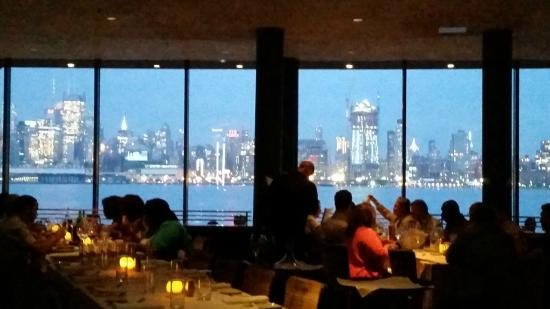
\includegraphics[width=.7\textwidth]{chart-house.jpg}
\end{center}

\begin{flushright}
\tiny\url{https://www.tripadvisor.com/LocationPhotoDirectLink-g46907-d7289700-i131403948}
\end{flushright}
\end{frame}


\begin{frame}
\frametitle{Ongoing Work}

Complement syntax with \textit{lexical} semantics to make up for differences.

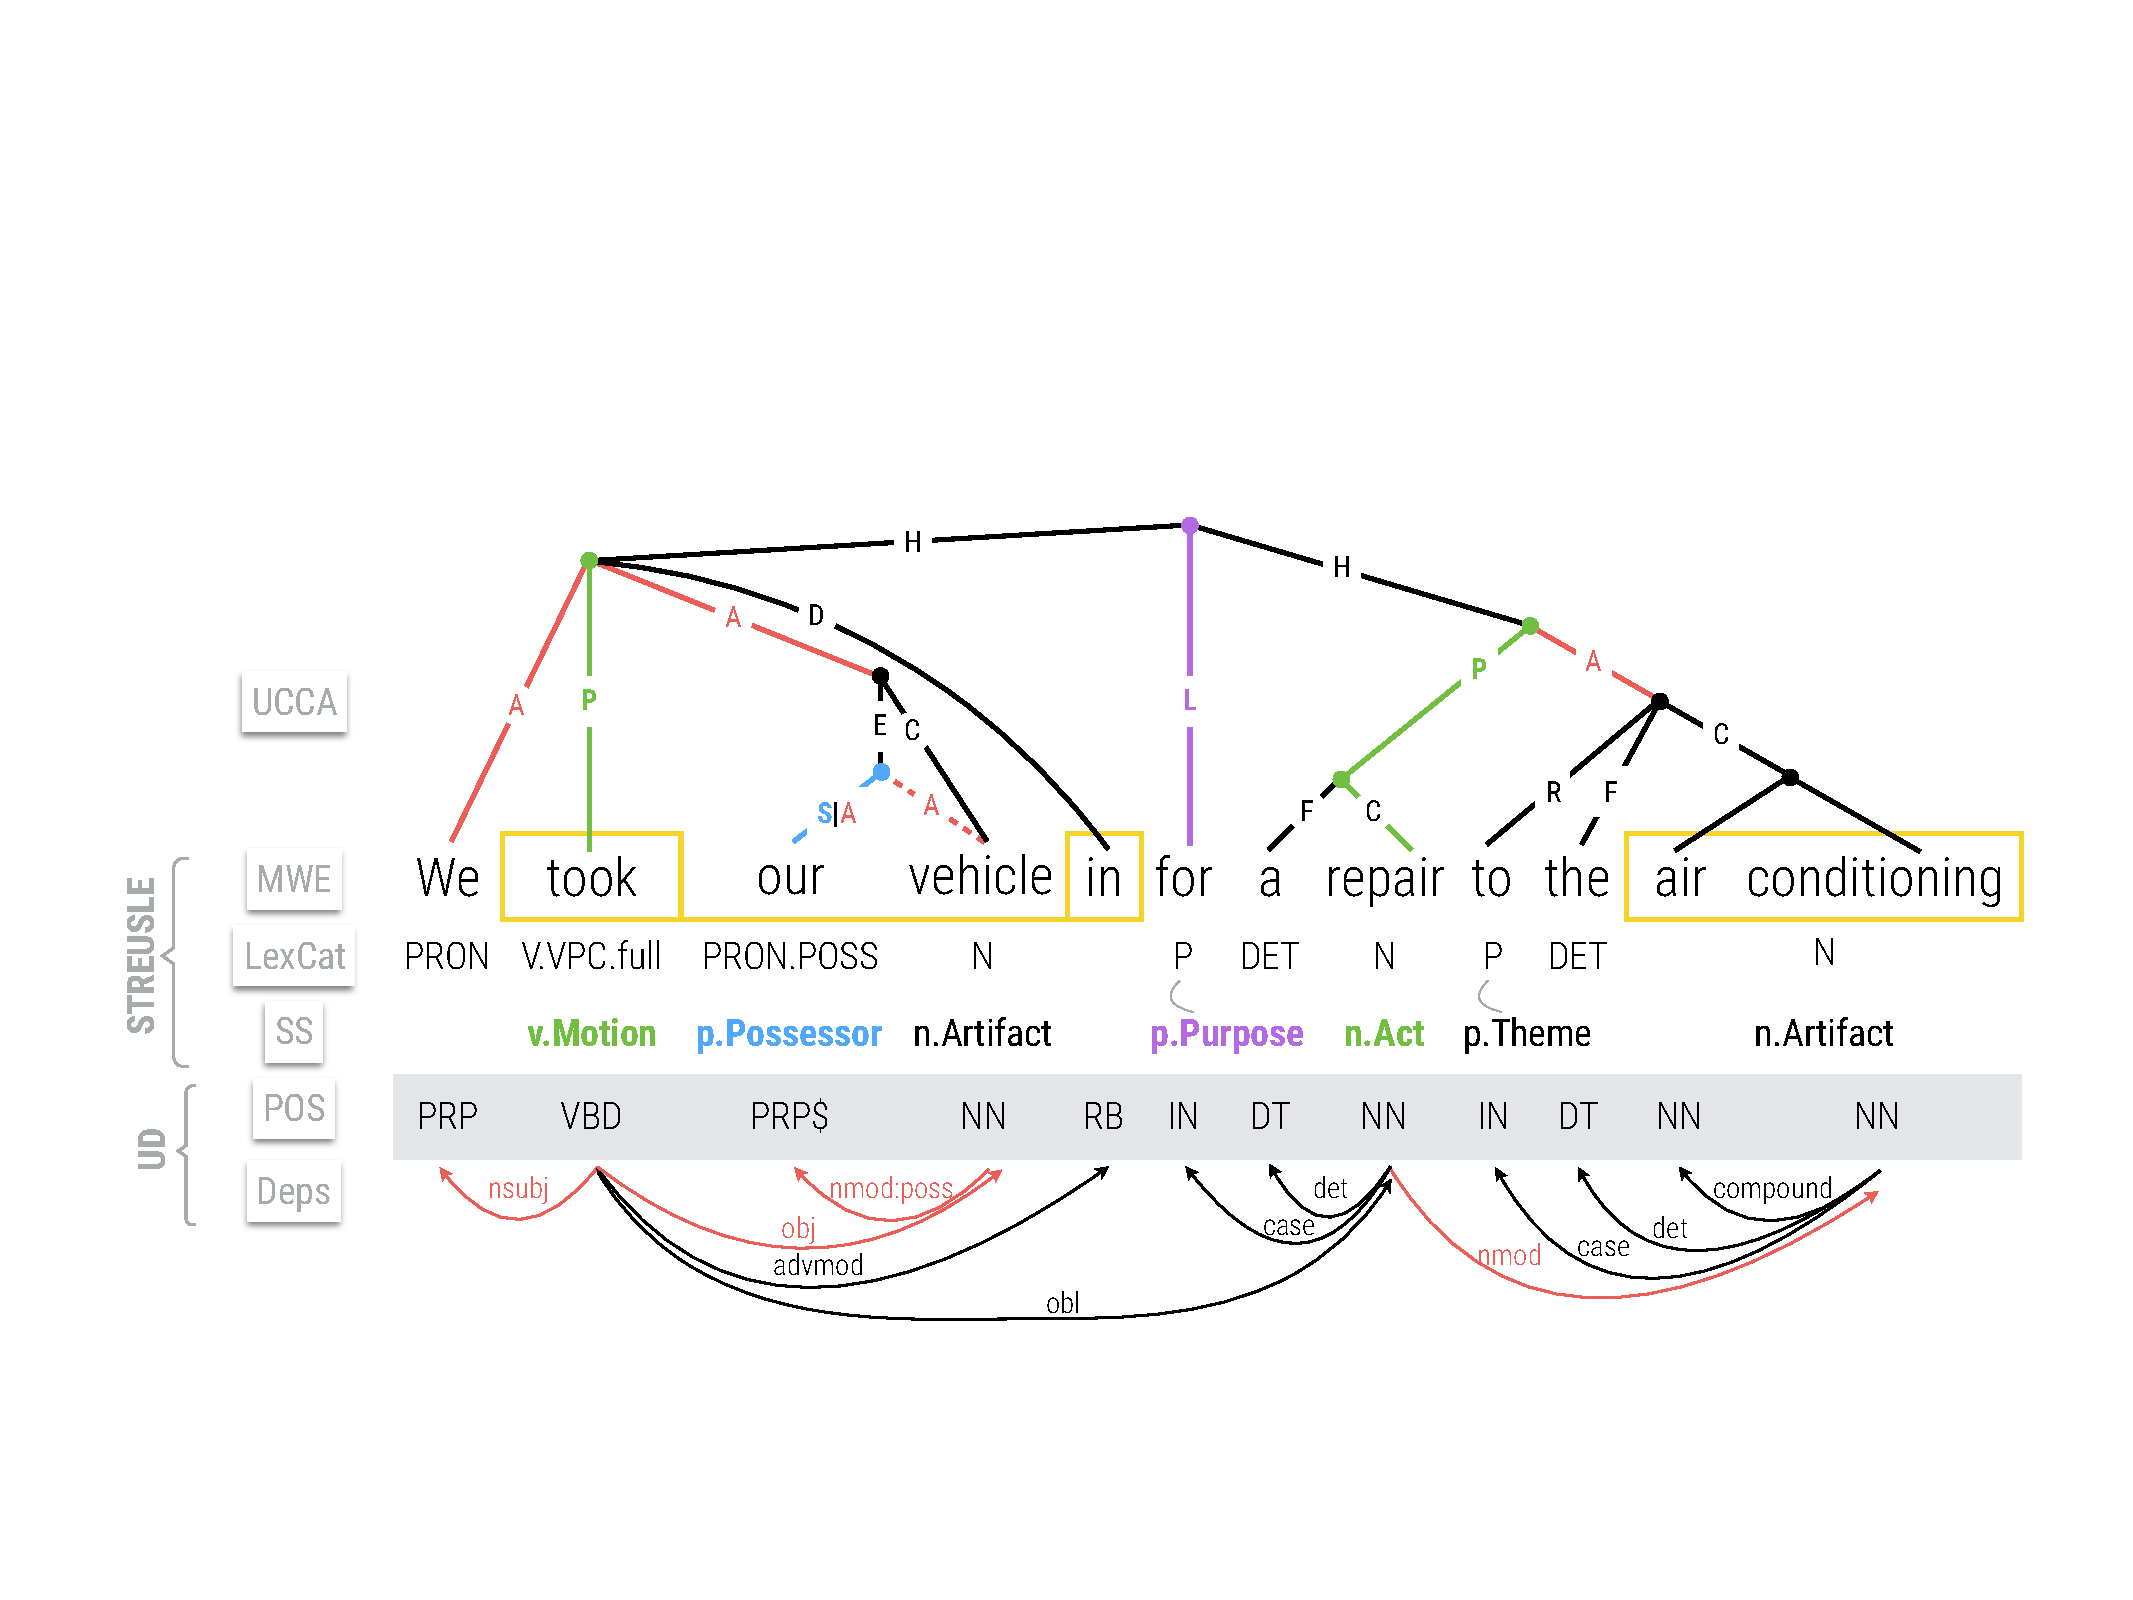
\includegraphics[width=\textwidth]{ex-ucca-streusle.pdf}

\end{frame}


\begin{frame}
\frametitle{Conclusion}
\begin{itemize}
 \item Meaning representation is valuable for language understanding.\pause
 \item Transition-based parsers excel across frameworks and languages.\pause
 \item Cross-framework unification by multi-task and linguistic analysis.
\end{itemize}

\vfill
\begin{flushright}
Thanks!
\end{flushright}

\end{frame}

\begin{frame}[allowframebreaks]
\frametitle{References}
\bibliographystyle{plainnat}
\tiny\bibliography{references}
\end{frame}

\begin{frame}
\frametitle{Structural Properties}
\noindent
\centering
\begin{minipage}{.5\linewidth}{\centering
(1) {\color{blue} non-terminal nodes}

\scalebox{.8}{
  \begin{tikzpicture}[level distance=12mm, sibling distance=16mm, ->, thick,
      every node/.append style={midway},
      edge from parent/.append style={nodes={font=\scriptsize}}]
    \node (ROOT) [fill=blue, circle] {}
      child {node [fill=blue, circle] {}
      {
        child {node {John} edge from parent node[left] {C}}
        child {node {and} edge from parent node[left] {N}}
        child {node {Mary} edge from parent node[right] {C}}
      } edge from parent node[left] {A} }
      child {node {went} edge from parent node[left] {P}}
      child {node {home} edge from parent node[right] {A}}
      ;
  \end{tikzpicture}
  }}
\end{minipage}
\hfill
\begin{minipage}{.48\linewidth}{\centering
(2) {\color{red} discontinuity}

\scalebox{.8}{
  \begin{tikzpicture}[level distance=12mm, sibling distance=2cm, ->, thick,
      every node/.append style={midway},
      edge from parent/.append style={nodes={font=\scriptsize}}]
    \node (ROOT) [fill=black, circle] {}
      child {node {John} edge from parent node[left] {A}}
      child {node [fill=black, circle] {}
      {
      	child {node {gave} edge from parent node[left] {C}}
      	child {node (everything) {everything} edge from parent[white]}
      	child {node {up} edge from parent node[right] {C}}
      } edge from parent node[right] {P} }
      ;
    \draw[bend right,->,red,very thick] (ROOT) to[out=-20, in=180] node [left] {\scriptsize A} (everything);
  \end{tikzpicture}
  }}
\end{minipage}

\vfill
(3) {\color{orange} reentrancy}

\scalebox{.8}{
\begin{tikzpicture}[level distance=14mm, sibling distance=17mm, ->, thick,
    edge from parent/.append style={nodes={font=\scriptsize}}]
    \node (ROOT) [fill=black, circle] {}
      child {node (After) {After} edge from parent node[left] {L\;}}
      child {node (graduation) [fill=black, circle] {}
      {
        child {node {graduation} edge from parent node[left] {P}}
      } edge from parent node[left] {H} }
      child {node {,} edge from parent node[right] {U}}
      child {node (moved) [fill=black, circle] {}
      {
        child {node (John) {John} edge from parent node[left] {A}}
        child {node {moved} edge from parent node[left] {P}}
        child {node [fill=black, circle] {}
        {
          child {node {to} edge from parent node[left] {R}}
          child {node {Copenhagen} edge from parent node[right] {C}}
        } edge from parent node[right] {A} }
      } edge from parent node[right] {H} }
      ;
    \draw[dashed,->,orange,very thick] (graduation) to node [auto] {\scriptsize A} (John);
\end{tikzpicture}}
\end{frame}


\begin{frame}
\frametitle{Data Statistics}
\centering
\def\arraystretch{1.5}
\begin{tabular}{l|r|rrr|r}
    & \multicolumn{1}{c|}{Wiki} & \multicolumn{3}{c|}{20K} & \multicolumn{1}{c}{EWT} \\
    & \multicolumn{1}{c|}{en} & \multicolumn{1}{c}{en} & \multicolumn{1}{c}{fr} & \multicolumn{1}{c|}{de} & \multicolumn{1}{c}{en} \\
    \hline
    \# sentences&5,141&492&492&6,514&3,520 \\
    \# tokens&158,739&12,638&13,021&144,529&51,042 \\
    \hline
    \# {\color{blue} non-terminal nodes}&62,002&4,699&5,110&51,934&18,156 \\
    \% {\color{red}discontinuous}&1.71&3.19&4.64&8.87&3.87 \\
    \% {\color{orange}reentrant}&1.84&0.89&0.65&0.31&0.83 \\
    \hline
    \# edges&208,937&16,803&17,520&187,533&60,739 \\
    \% primary&97.40&96.79&97.02&97.32&97.32 \\
    \% remote&2.60&3.21&2.98&2.68&2.68
\end{tabular}
\end{frame}


\begin{frame}
\frametitle{Evaluation}
\begin{adjustbox}{frame,scale=.75,center}
    \begin{tikzpicture}[level distance=12mm, sibling distance=15mm, ->,
        every circle node/.append style={fill=black},
        edge from parent/.append style={nodes={font=\scriptsize}},
        edge from parent path={(\tikzparentnode.center) -- (\tikzchildnode.north)}]
      \tikzstyle{word} = [font=\rmfamily,color=black]
      \node at (0,.7) {True (human-annotated) graph};
      \node (ROOT) at (0,0) [circle] {}
        child {node (After) [word] {After} edge from parent node[left] {L}}
        child {node (graduation) [circle] {}
        {
          child {node [word] {graduation} edge from parent node[left] {P}}
        } edge from parent node[left] {H} }
        child {node [word] {,} edge from parent node[right] {U}}
        child {node (moved) [circle] {}
        {
          child {node (John) [word] {John} edge from parent node[left] {A}}
          child {node [word] {moved} edge from parent node[left] {P}}
          child {node [circle] {}
          {
            child {node [word] {to} edge from parent node[left] {R}}
            child {node [word] {Copenhagen} edge from parent node[right] {C}}
          } edge from parent node[right] {A} }
        } edge from parent node[right] {H} }
        ;
      \draw[dashed,->] (graduation) to node [auto] {\scriptsize A} (John);
      \node at (8,.7) {Automatically predicted graph for the same text};
      \node (ROOT_) at (7,0) [circle] {}
        child {node (After_) [word] {After} edge from parent node[left] {L}}
        child {node (graduation_) [circle] {}
        {
          child[alt=<2>{red}{}] {node [word] {graduation} edge from parent node[left] {S}}
        } edge from parent node[left] {H} }
        child {node [word] {,} edge from parent node[right] {U}}
        child {node (moved) [circle,xshift=3mm,yshift=-7mm] {}
        {
          child {node (John_) [word] {John} edge from parent node[left] {A}}
          child {node [word] {moved} edge from parent node[left] {P}}
          child[alt=<2>{red}{}] {node [word] {to} edge from parent node[left] {F}}
          child[alt=<2>{red}{}] {node (Copenhagen_) [word] {Copenhagen} edge from parent node[right] {A}}
        } edge from parent node[right] {H} }
        ;
      \draw[dashed,->] (graduation_) to node [auto] {\scriptsize A} (John_);
      \draw[bend left,dashed,->,alt=<2>{red}{}] (graduation_) to[in=90] node [auto] {\scriptsize A} (Copenhagen_);
    \end{tikzpicture}
\end{adjustbox}
\vfill

\begin{enumerate}
  \item Match primary edges between the graphs by terminal yield and label.
  \item Calculate \textbf{precision, recall and F1} scores.
  \item Repeat for remote edges.
\end{enumerate}

\pause
\vfill
\begin{adjustbox}{center}
    \begin{tabular}{c|c|c}
        \multicolumn{3}{l}{Primary} \\
        \textbf{P} & \textbf{R} & \textbf{F1} \\ \hline
        $\frac69=67\%$ & $\frac6{10}=60\%$ & 64\%
    \end{tabular}
    \hspace{1cm}
    \begin{tabular}{c|c|c}
        \multicolumn{3}{l}{Remote} \\
        \textbf{P} & \textbf{R} & \textbf{F1} \\ \hline
        $\frac12=50\%$ & $\frac11=100\%$ & 67\%
    \end{tabular}
\end{adjustbox}
\end{frame}

\end{document}
